\documentclass[11pt,a4paper]{article}
\usepackage[hyperref]{emnlp-ijcnlp-2019}
\usepackage{times}
\usepackage{latexsym}
\usepackage{url}
%\usepackage[T1]{fontenc}

\aclfinalcopy % Uncomment this line for the final submission

%\setlength\titlebox{5cm}
% You can expand the titlebox if you need extra space
% to show all the authors. Please do not make the titlebox
% smaller than 5cm (the original size); we will check this
% in the camera-ready version and ask you to change it back.

\newcommand\BibTeX{B{\sc ib}\TeX}
\newcommand\confname{EMNLP-IJCNLP 2019}
\newcommand\conforg{SIGDAT}


\usepackage{xspace,mfirstuc,tabulary}
\newcommand{\ex}[1]{{\sf #1}}
\usepackage{graphicx}
\usepackage{tabularx}
\usepackage{array}
\newcolumntype{P}[1]{>{\centering\arraybackslash}p{#1}}
\newcolumntype{Y}{>{\raggedright\arraybackslash}X}
\newcolumntype{?}{!{\vrule width 1pt}}
\newcolumntype{h}{!{\vrule width 0.7pt}}
\usepackage[fleqn]{amsmath}
\usepackage{amsfonts}
\usepackage{algorithm2e}
\usepackage[boldmath]{numprint}
\usepackage{url}
\usepackage[caption=false,font=footnotesize]{subfig}
\usepackage{float}
%\captionsetup[subfigure]{margin=0pt}
\usepackage{booktabs}
\usepackage{tikz}
\usepackage{todonotes}

\makeatletter
\makeatother %some sort of hack related to the symbol @

\newcommand{\bs}{\boldsymbol} 
\DeclareMathOperator*{\argmax}{\arg\!\max\!} %argmax operator
\newcommand{\wrtd}{\mathrm{d}}

\newcommand{\rough}[0]{\color{purple}}

\newcommand{\Arrow}[1]{\parbox{#1}{\tikz{\draw[->](0,0)--(#1,0)}} }

%%%%%%%%%%%%%%%%%%%%%%%%%%%%%%%%%%%%%%%%%%%%%%%%%%%%%%%%%%%%%%%%%

%\title{Bayesian Ensembles of Crowds and Deep Learners for Sequence Tagging}
%Multiple Unreliable Text Annotators}
\title{Appendix for: A Bayesian Approach for Sequence Tagging with Crowds}

\author{Edwin Simpson and Iryna Gurevych\\
  Ubiquitous Knowledge Processing Lab \\
  Department of Computer Science \\
  Technische Universit\"at Darmstadt \\
  \url{https://www.ukp.tu-darmstadt.de} \\
  {\tt \{simpson,gurevych\}@ukp.informatik.tu-darmstadt.de}
}

\begin{document}

\maketitle

% up to eight (8) pages of content, plus unlimited pages for references
% Each EMNLP 2018 submission can be accompanied by a single PDF appendix <--put equations in here
% + one .tgz or .zip archive containing software, and one .tgz or .zip archive containing data
% make sure that these are also anonymized.

% This paper shows how common annotator models for crowdsourcing can be seen as extensions of one another
% particularly in small-data scenarios that occur at the beginning of a crowdsourcing process.
%We publish our code to encourage adaptation and reuse.

\section{Discussion of Variational Approximation}

In Equation 12 of the main paper,
each subset of latent variables has a variational factor of the form 
$\ln q(z) = \mathbb{E}[\ln p(z | \bs c, \neg z)]$, 
where $\neg z$ contains all the other latent variables excluding $z$.
We perform approximate inference by
%we optimize Equation \ref{eq:vb_posterior} 
using coordinate ascent to update each variational factor, $q(z)$, in turn,
taking expectations with respect to the current estimates of the other variational factors.
%(see Algorithm \ref{al:vb_bac}).
Each iteration reduces the KL-divergence between the true and approximate posteriors
of Equation 12, and hence optimises a lower bound on the 
log marginal likelihood, also called the evidence lower bound or ELBO
~\cite{Bishop2006,attias_advances_2000}.

\paragraph{Conjugate distributions: }The prior distributions chosen for our generative model are conjugate to the distributions over the
latent variables and model parameters, 
meaning that each $q(z)$ is the same type of distribution
as the corresponding  prior distribution defined in Section 4.
The parameters of each variational distribution are computed in terms  of 
expectations over the other subsets of variables.


\begin{figure*}[t]
\begin{minipage}[b][1cm][l]{0.2\textwidth} 
BSC-seq, \\
previous label = I:
\end{minipage}
  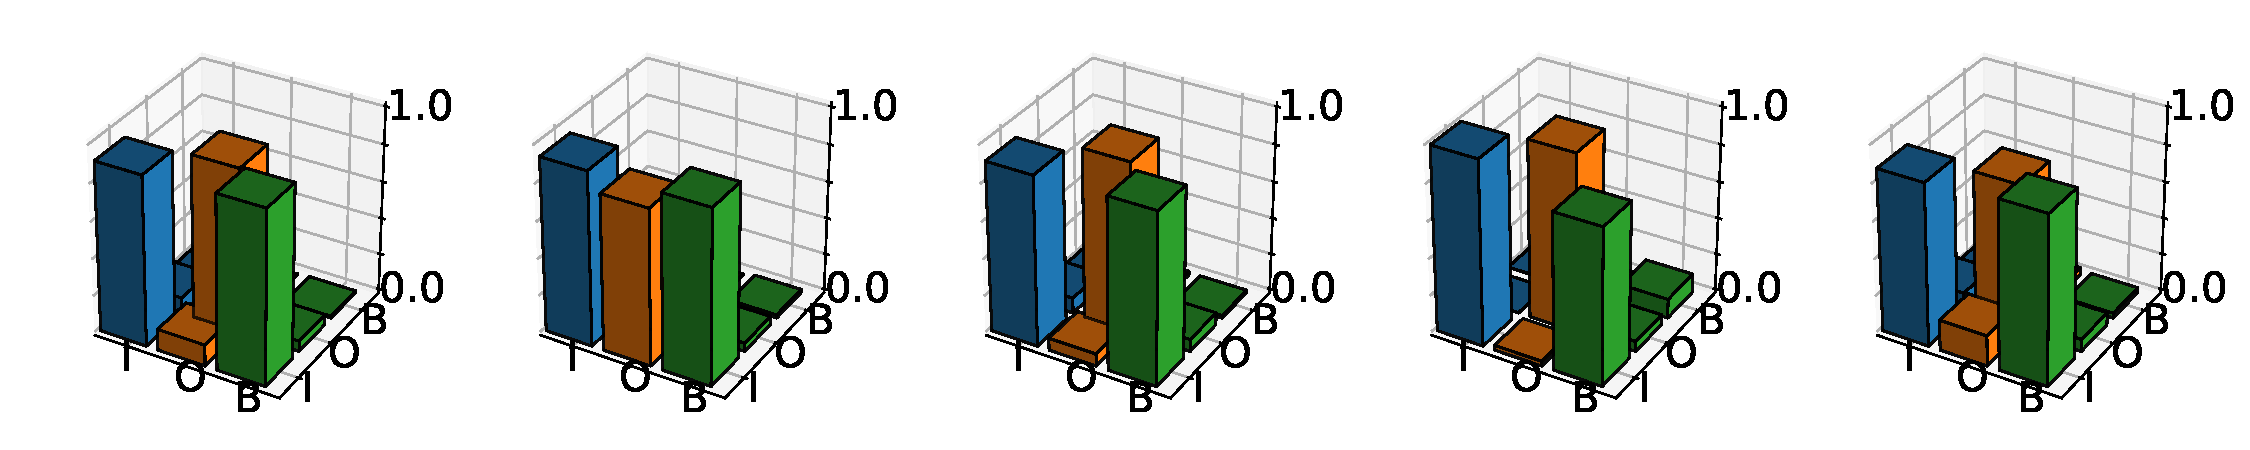
\includegraphics[width=0.8\textwidth, clip=True, trim=10 0 0 10]{figures/worker_models/seq_prev0}
\\
\begin{minipage}[b][1cm][l]{0.2\textwidth} 
BSC-seq, \\
previous label = O:
\end{minipage}
  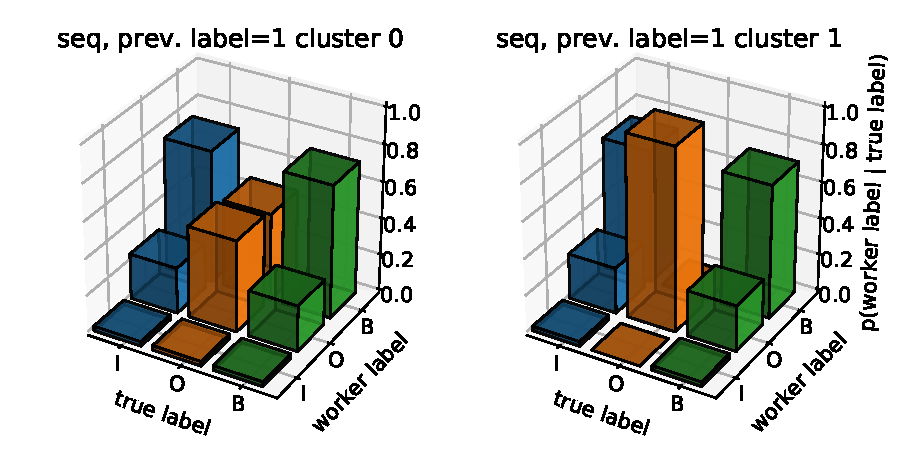
\includegraphics[width=0.8\textwidth, clip=True, trim=10 0 0 23]{figures/worker_models/seq_prev1}
\\
\begin{minipage}[b][1cm][l]{0.2\textwidth} 
BSC-seq,\\
 previous label = B:
\end{minipage}
  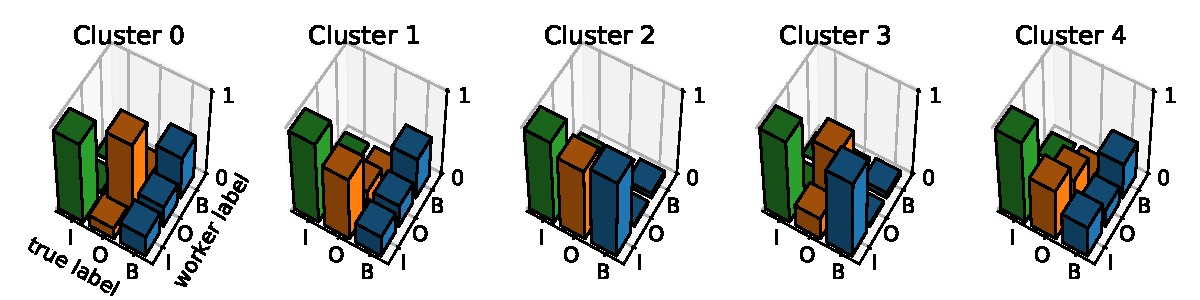
\includegraphics[width=0.8\textwidth, clip=True, trim=10 0 0 23]{figures/worker_models/seq_prev2}
\\
\caption{Clusters of confusion matrix representations from BSC-seq trained on PICO. 
}
\label{fig:anno_models_2}
\end{figure*}

\section{Update Equations for the Forward-Backward Algorithm}

For the true labels, $\bs t$, the variational factor is:
 \begin{flalign}
& \ln q(\bs t_n) \!=\! 
% \sum_{n=1}^N \sum_{\tau=1}^{L_n} 
% \sum_{s=1}^S \mathbb{E}%_{\bs B,\bs d^{(s)}} \!\left[ 
% \ln \!B^{(s)}\!\!\left(t_{n,\tau},d_{n,\tau}^{(s)},d_{n,\tau\!-\!1}^{(s)}\!\right) %\right]
% %\bigg\{ \mathbb{E}%_{\bs T} \left[ 
% %\ln T_{t_{n,\tau\!-\!1}, t_{n,\tau}} %\right] 
% &&\nonumber \\
%+ 
\sum_{n=1}^N \sum_{\tau=1}^{L_n} \sum_{k=1}^K  \mathbb{E}%_{\bs A} \left[ 
\ln \!A^{(k)}\left(t_{n,\tau},c_{n,\tau}^{(k)},c_{n,\tau-1}^{(k)}\right) %\right]  
&\nonumber\\
&+ \mathbb{E}\ln T_{t_{n,\tau-1}, t_{n,\tau}}+\mathrm{const}. & \label{eq:qstar_t}
 \end{flalign}
 
% TODO move all this to the appendix
 The forward-backward algorithm consists of two passes. 
 The \emph{forward pass} for each document, $n$, starts from $\tau=1$
 and computes:% for each value of $\tau$:
 % the posterior given crowdsourced annotations for tokens $\leq\tau$. 
 \begin{flalign}
   & \ln r^{-}_{n,\tau,j} = \ln \sum_{\iota=1}^J \left\{ r^{-}_{n,\tau-1,\iota} \mathrm{e}^{\mathbb{E}\ln T_{\iota,j}} \right\} + ll_{n,\tau}(j), & \nonumber \\
% \end{flalign}
%  where the log likelihood $ll(j,n,\tau)$ of the annotations for token $\tau$ in document $n$ giventr
%  label $j$ is:
% \begin{flalign} 
   & ll_{n,\tau}(j) = \sum_{k=1}^K \mathbb{E}%_{\bs A}
   \ln A^{(k)}\left(j, c_{n,\tau}^{(k)}, c_{n,\tau\!-\!1}^{(k)} \right) & 
   %+  \sum_{s=1}^S
%    & \nonumber \\
%    &  \sum_{i=1}^J\sum_{\iota=1}^J \mathbb{E}%_{\bs B}
%    \ln B^{(s)} \!\left(j, i, \iota \right)  
%    \hat{d}_{n,\tau}^{(s)}(i) \hat{d}_{n,\tau-1}^{(s)}(\iota), & 
 \end{flalign}
 %where $\hat{d}_{n,\tau}^{(s)}(i)$ is %the probability of label $d_{n,\tau}^{(s)}$ produced 
% by the sequence tagger $s$, which we explain in more detail below (see Equation \ref{eq:hatp}).
%defined below in Equation \ref{eq:hatp}, and 
where $r^{-}_{n,0,\iota}  = 1$ where $\iota=$`O' and $0$ otherwise.
The \emph{backwards pass} starts from $\tau=L_n$ and scrolls backwards, computing:
%at each token computing the likelihoods of the annotations from $\tau+1$ to $L_n$:
 \begin{flalign}
  & \ln \lambda_{n,L_n,j} = 0, \hspace{1cm}
   \ln \lambda_{n,\tau,j} = \ln\sum_{\iota=1}^J \exp \big\{ 
   & \nonumber \\
& \ln \lambda_{i,\tau+1,\iota} + \mathbb{E}\ln T_{j,\iota} + ll_{n,\tau+1}(\iota) \big\} .&
 \end{flalign}
% To avoid $r^{-}_{n,\tau,j}$ and $\lambda_{n,\tau,j}$ becoming too small over a long sequence, we normalize them after each iteration of the forward and backward pass
% by dividing by their sum over $j$.
 By %taking the exponents and 
 applying Bayes' rule, we arrive at $r_{n,\tau,j}$ and $s_{n,\tau,j,\iota}$:
 \begin{flalign}
  & r_{n,\tau,j} = \frac{r^{-}_{n,\tau,j}\lambda_{n,\tau,j}}{\sum_{j'=1}^J r^{-}_{n,\tau,j'}\lambda_{n,\tau,j'}} &\\
%} {\sum_{\iota=1}^J \sum_{\iota'=1}^J  
%  r^{-}_{n,\tau\!-\!1,\iota}\lambda_{n,\tau,\iota'} \exp\mathbb{E}[\ln T_{\iota,\iota'}] 
% + ll(\iota',n,\tau)  } . &
& s_{n,\tau,j,\iota} = \frac{ \tilde{s}_{n,\tau,j,\iota} }{ \sum_{j'=1}^J\sum_{\iota'=1}^J  \tilde{s}_{n,\tau,j',\iota'} } & \\
  & \tilde{s}_{n,\tau,j,\iota} =  r^{-}_{n,\tau-1,j} \lambda_{n,\tau,\iota} \exp\{\mathbb{E}\ln T_{j,\iota}
+ ll_{n,\tau}(\iota)\}. & \nonumber 
 \end{flalign}
 
 Each row of the transition matrix has the factor:
\begin{flalign}
& \ln q(\bs T_{j}) 
  %= \sum_{\iota=1}^J N_{j,\iota}  + \ln \mathrm{Dir}(\bs T_j | \bs\gamma_j) + \mathrm{const} & \nonumber\\
= \ln \mathrm{Dir}\left(\left[ N_{j,\iota} + \gamma_{j,\iota}, \forall \iota \in \{1,..,J\} \right]\right), &
\end{flalign}
where $N_{j,\iota} = \sum_{n=1}^N \sum_{\tau=1}^{L_n}  s_{n,\tau,j,\iota}$ is the expected number of times that label $\iota$ follows label $j$.  
%The variational factor $q(\bs t)$ requires the following expectation:
The forward-backward algorithm requires expectations of $\ln \bs T$ that can be computed using standard equations for a Dirichlet distribution:
 \begin{flalign}
& \mathbb{E}\ln T_{j,\iota} = \Psi\!\left(N_{j,\iota} \!\!+ \gamma_{j,\iota}\right) 
 - \Psi\!\left(\sum_{\iota=1}^J (N_{j,\iota} \!\!+ \gamma_{j,\iota}) \!\right), &
\end{flalign}
 where $\Psi$ is the digamma function.
 
 
 
%\textbf{Variational factors for} $\bs A$ and $\bs B$:
The variational factor for each annotator model is a distribution over its parameters, 
which differs between models.
For \emph{seq}, the variational factor is:
 \begin{flalign}
  & \ln q\!\left(\! A^{(k)}\!\right) %= \sum_{j=1}^J  \sum_{l=1}^J \bigg\{ \sum_{m=1}^J N_{j,l,m}^{(k)}\ln\pi_{j,l,m}^{(k)} & \nonumber\\
 % & \hspace{2.7cm} 
 % + \ln p\left(\bs\pi_{j,l}^{(k)} | \bs \alpha_{j,l}^{(k)} \right) \bigg\} + \mathrm{const}, & \nonumber \\
  \!=\! \sum_{j=1}^J \! \sum_{l=1}^J \!\mathrm{Dir}\! \left(\left[ \bs N_{j,l,m}^{(k)} \! 
 %+ \alpha_{j,l,m}^{(k)}, \! 
 %\right.\right.\nonumber&\\
%&  \hspace{3.5cm} \left.\left.
\forall m \! \in \! \{1,..,J\} \!\right] \right) & \nonumber \\
& N^{(k)}_{j,l,m} \!\!=\!  \alpha_{j,l,m}^{(k)} \!\!\! + \!\sum_{n=1}^N \!\sum_{\tau=1}^{L_n} \!
r_{n,\tau,j} \delta_{l,c^{(k)}_{n,\tau\!-\!1}}\!\delta_{m,c^{(k)}_{n, \!\tau}}, \!& 
\end{flalign}
 where $\delta$ is the Kronecker delta. 
% For the \emph{CM} model, the variational factor is simplified to:
%  \begin{flalign}
%   & \ln q\left( A^{(k)}\right) = \sum_{j=1}^J  \mathrm{Dir} \bigg( \bigg[ \sum_{n=1}^N \sum_{\tau=1}^{L_n} r_{n,\tau,j} \delta_{m,c^{(k)}_{n,\tau}} 
%   & \nonumber \\ 
% & \hspace{2.0cm} + \alpha_{j,m}^{(k)}, \! \forall m \! \in \! \{1,..,J\} \bigg] \bigg) .
% \end{flalign}
For \emph{CM}, \emph{MACE}, \emph{CV} and \emph{acc}, the factors follow a similar pattern of summing pseudo-counts of correct and incorrect answers. 
%For reasons of space, we omit the equations for these variants. 

\section{Visualising Annotator Models}

Figure \ref{fig:anno_models_2} provides an alternative visualisation of the \textit{seq} models inferred by BSC-seq for annotators in the PICO dataset.
The annotators were clustered as described in Section 6 of the main paper,
and the mean confusion matrices for each cluster are plotted in Figure \ref{fig:anno_models_2} using 3D plots to emphasise the differences between 
the likelihoods of annotators in each cluster providing a particular label 
given the true label value.

%%%%%%%%%%%%%%%%%%%%%%%%%%%%%%%%%%%%%%%%%%%%%%%%%%%%%%%%%%%%%%%%%%%%%%%%%%%%%%%%

%\section*{Acknowledgments}

% \addcontentsline{toc}{chapter}{Bibliography}
%\bibliographystyle{apalike}
% \bibliographystyle{IEEEtran}
\bibliographystyle{acl_natbib}
\bibliography{simpson}

%\appendix
%\section{Update Equations for the Forward-Backward Algorithm}
% TODO move all this to the appendix
 The forward-backward algorithm consists of two passes. 
 The \emph{forward pass} for each document, $n$, starts from $\tau=1$
 and computes:% for each value of $\tau$:
 % the posterior given crowdsourced annotations for tokens $\leq\tau$. 
 \begin{flalign}
   & \ln r^{-}_{n,\tau,j} = \ln \sum_{\iota=1}^J \left\{ r^{-}_{n,\tau-1,\iota} \mathrm{e}^{\mathbb{E}\ln T_{\iota,j}} \right\} + ll_{n,\tau}(j), & \nonumber \\
% \end{flalign}
%  where the log likelihood $ll(j,n,\tau)$ of the annotations for token $\tau$ in document $n$ given
%  label $j$ is:
% \begin{flalign} 
   & ll_{n,\tau}(j) = \sum_{k=1}^K \mathbb{E}%_{\bs A}
   \ln A^{(k)}\left(j, c_{n,\tau}^{(k)}, c_{n,\tau\!-\!1}^{(k)} \right) & 
   %+  \sum_{s=1}^S
%    & \nonumber \\
%    &  \sum_{i=1}^J\sum_{\iota=1}^J \mathbb{E}%_{\bs B}
%    \ln B^{(s)} \!\left(j, i, \iota \right)  
%    \hat{d}_{n,\tau}^{(s)}(i) \hat{d}_{n,\tau-1}^{(s)}(\iota), & 
 \end{flalign}
 %where $\hat{d}_{n,\tau}^{(s)}(i)$ is %the probability of label $d_{n,\tau}^{(s)}$ produced 
% by the sequence tagger $s$, which we explain in more detail below (see Equation \ref{eq:hatp}).
%defined below in Equation \ref{eq:hatp}, and 
where $r^{-}_{n,0,\iota}  = 1$ where $\iota=$`O' and $0$ otherwise.
The \emph{backwards pass} starts from $\tau=L_n$ and scrolls backwards, computing:
%at each token computing the likelihoods of the annotations from $\tau+1$ to $L_n$:
 \begin{flalign}
  & \ln \lambda_{n,L_n,j} = 0, \hspace{1cm}
   \ln \lambda_{n,\tau,j} = \ln\sum_{\iota=1}^J \exp \big\{ 
   & \nonumber \\
& \ln \lambda_{i,\tau+1,\iota} + \mathbb{E}\ln T_{j,\iota} + ll_{n,\tau+1}(\iota) \big\} .&
 \end{flalign}
% To avoid $r^{-}_{n,\tau,j}$ and $\lambda_{n,\tau,j}$ becoming too small over a long sequence, we normalize them after each iteration of the forward and backward pass
% by dividing by their sum over $j$.
 By %taking the exponents and 
 applying Bayes' rule, we arrive at $r_{n,\tau,j}$ and $s_{n,\tau,j,\iota}$:
 \begin{flalign}
  & r_{n,\tau,j} = \frac{r^{-}_{n,\tau,j}\lambda_{n,\tau,j}}{\sum_{j'=1}^J r^{-}_{n,\tau,j'}\lambda_{n,\tau,j'}} &\\
%} {\sum_{\iota=1}^J \sum_{\iota'=1}^J  
%  r^{-}_{n,\tau\!-\!1,\iota}\lambda_{n,\tau,\iota'} \exp\mathbb{E}[\ln T_{\iota,\iota'}] 
% + ll(\iota',n,\tau)  } . &
& s_{n,\tau,j,\iota} = \frac{ \tilde{s}_{n,\tau,j,\iota} }{ \sum_{j'=1}^J\sum_{\iota'=1}^J  \tilde{s}_{n,\tau,j',\iota'} } & \\
  & \tilde{s}_{n,\tau,j,\iota} =  r^{-}_{n,\tau-1,j} \lambda_{n,\tau,\iota} \exp\{\mathbb{E}\ln T_{j,\iota}
+ ll_{n,\tau}(\iota)\}. & \nonumber 
 \end{flalign}


\end{document}
